\documentclass[t,ngerman]{beamer}
\listfiles
\usefonttheme{professionalfonts}
\IfFileExists{beamerthemesl-it.sty}{%
  \usetheme{sl-it}
  \useoutertheme{sl-split}
  \usepackage{sl-listings}
}{%
  \usetheme{Luebeck}
  \usepackage{babel}
  \usepackage{listings}
}
\usepackage[backend=biber%
  ,language=german]{biblatex}
\addbibresource{biblio.bib}
\usepackage{csquotes}
\usepackage{hologo}
\usepackage{tikz}
\usepackage{graphicx}
\graphicspath{{./img/}}
\usepackage{ifluatex}
\ifluatex%
\else%
  \usepackage[utf8]{inputenc}%
\fi

\newcommand\examplefile[2]{%
  \footnotesize\centering%
  \href{#2}{%
    
\includegraphics[height=.75\baselineskip]{examplefile}~\textsl{#1}%
  }
}

\author{Stephan Lukasczyk}
\title{\LaTeX{} im Uni-Alltag}
\subtitle{Ein \enquote{kleiner} \"Uberblick}
\date{15.~Januar 2014}
\institute{
\includegraphics[width=3cm]{ieee-logo}\\%
  IEEE Student Branch Passau}
\begin{document}

\begin{frame}
  \titlepage
  \begin{textblock}{4}(0.67,0.4)
    
\includegraphics[width=4cm]{lion}
  \end{textblock}
\end{frame}

\begin{frame}
  \frametitle{Agenda}
  \tableofcontents
\end{frame}

\section{Einführung}

\subsection{The Name of the Game}

\begin{frame}
  \frametitle{The Name of the Game}
  \framesubtitle{Just drop a view names}
  \begin{itemize}
  \item \TeX
    \begin{itemize}
    \item Donald E. Knuth, 1978
    \item Aktuell \TeX{} 3.1415926 (März~2008)
    \item Textsatzsystem mit eingebauter\\
      Makrosprache
    \item \enquote{The \TeX{}book}
    \end{itemize}
  \item \LaTeX
    \begin{itemize}
    \item Leslie Lamport, Anfang 1980er
    \item Aktuell \hologo{LaTeX2e}
    \item Makropaket für \TeX
    \item Meistverwendetste \TeX-Variante
    \item Unzählige Literatur
    \end{itemize}
  \item CTAN (Comprehensive \TeX{} Archive Network)
    \begin{itemize}
    \item über 4\,600 Pakete
    \item \texttt{CTAN://<pkg>} für \href{http://ctan.org}{\texttt{http://ctan.org/<pkg>}}
    \end{itemize}
  \end{itemize}
  \begin{textblock}{3}(0.72,0.17)
    \href{https://en.wikipedia.org/wiki/File:KnuthAtOpenContentAlliance.jpg}{%
      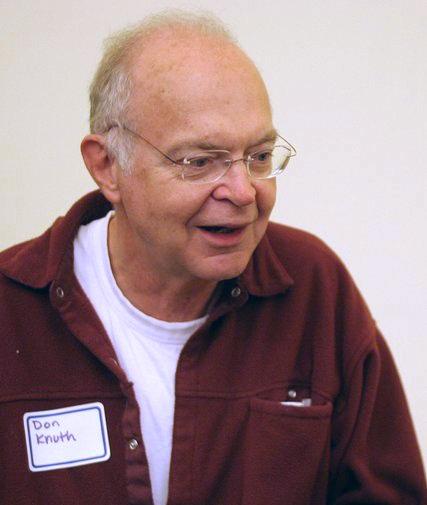
\includegraphics[width=3cm]{don-knuth}~%
      \rotatebox{90}{\tiny by Jacob Applebaum (CC-BY-SA 2.5)}%
    }
  \end{textblock}
  \begin{textblock}{3}(0.72,0.54)
    \href{https://en.wikipedia.org/wiki/File:Leslie_Lamport.jpg}{%
      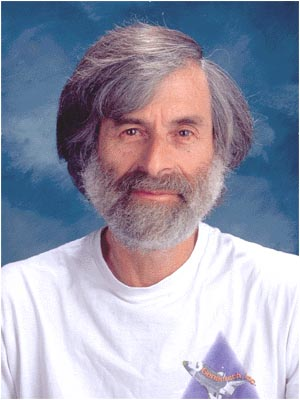
\includegraphics[width=3cm]{leslie-lamport}~%
      \rotatebox{90}{\tiny by Leslie Lamport}%
    }
  \end{textblock}
\end{frame}

\begin{frame}
  \frametitle{The Name of the Game (2)}
  \framesubtitle{Engines}
  \begin{itemize}
  \item \TeX\\
    7\,bit-ASCII, dvi-Ausgabe, v3.1415926
  \item pdf\TeX\\
    8\,bit-ASCII, dvi- oder pdf-Ausgabe, v1.40.14
  \item \hologo{XeTeX}\\
    UTF-8, Systemfonts (TTF, OTF), nur pdf-Ausgabe, schleppende
    Entwicklung, v0.9999.3
  \item \hologo{LuaTeX}\\
    UTF-8, Systemfonts (TTF, OTF), dvi- oder pdf-Ausgabe, Lua
    eingebettet, Arabischer Textsatz, v0.76
  \end{itemize}
\end{frame}

\subsection{Einführungen}

\begin{frame}
  \frametitle{Einführungen}
  \nocite{voss2012,l2short}
  \begingroup
  \printbibliography[heading=none]
  \endgroup
\end{frame}

\section{(Kryptische) Fehlermeldungen}

\subsection{Übliche Fehler}

\begin{frame}
  \frametitle{Tippfehler}
  \only<1->{%
    \begin{columns}[T]
      \begin{column}{.5\textwidth}
        \examplefile{examples/errors/typo.tex}
        \lstinputlisting[language={[LaTeX]TeX}]{examples/errors/typo.tex}
      \end{column}
      \begin{column}{.5\textwidth}
        Fehlermeldung:
        \lstinputlisting{examples/errors/typo.err}
      \end{column}
    \end{columns}
  }% End of \only<1->
  \only<2->{%
    \begin{itemize}
    \item Wahrscheinlich häufigster Fehler
    \item Tippfehler im Kommandonamen
    \item Kommando nicht definiert?
    \end{itemize}
    \begin{tikzpicture}[overlay]
      \draw[color=red,very thick] (2.85,3.3) circle (8pt);
    \end{tikzpicture}
  }
\end{frame}

\begin{frame}
  \frametitle{Überschreiben eines vorhandenen Kommandos}
    \begin{columns}[T]
      \only<1->{\begin{column}{.5\textwidth}
        \examplefile{examples/errors/renewcommand.tex}
        \lstinputlisting[language={[LaTeX]TeX}]{examples/errors/renewcommand.tex}
      \end{column}}
      \only<1>{\begin{column}{.5\textwidth}
        Fehlermeldung:
        \lstinputlisting{examples/errors/renewcommand.err}
      \end{column}}
      \only<2->{\begin{column}{.5\textwidth}
        Fehlermeldung:
        \lstinputlisting[lastline=3]{examples/errors/renewcommand.err}
        \end{column}}
    \end{columns}
  \only<2->{%
    \begin{itemize}
    \item Kommando schon definiert
    \item Überschreiben mit \texttt{\textbackslash renewcommand}\\
      \alert{Vorsicht!} Nur wenn man wirklich weiß, was man tut!
    \end{itemize}
    \begin{tikzpicture}[overlay]
      \draw[color=red,very thick] (0,4.35) circle (8pt);
    \end{tikzpicture}
  }
\end{frame}

\subsection{Mathemodus}

\begin{frame}[fragile]
  \frametitle{Zeichen mit besonderer Bedeutung}
  \only<1->{%
  \begin{columns}[T]
    \begin{column}{.5\textwidth}
      \examplefile{examples/errors/underscore.tex}
      \lstinputlisting[language={[LaTeX]TeX}]{examples/errors/underscore.tex}
    \end{column}
    \begin{column}{.5\textwidth}
      Fehlermeldung:
      \lstinputlisting{examples/errors/underscore.err}
    \end{column}
  \end{columns}
  }% End of \only<1->
  \only<2->{%
    \begin{itemize}
    \item Fehler wegen \texttt{\color{red}\_}
    \item Startet automatisch Mathemodus\\
      $\Rightarrow$ fehlendes \texttt{\$} am Ende
    \item Lösung: \texttt{\color{red}\textbackslash\_} 
    \end{itemize}
    \begin{tikzpicture}[overlay]
      \draw[color=red,very thick] (3.9,4.5) circle (8pt);
    \end{tikzpicture}
  }% End of \only<2->
\end{frame}

\begin{frame}[fragile]
  \frametitle{Klammerchaos}
  \only<1->{%
    \begin{columns}[T]
      \begin{column}{.5\textwidth}
        \examplefile{examples/errors/leftright.tex}
        \lstinputlisting[language={[LaTeX]TeX}]{examples/errors/leftright.tex}
      \end{column}
      \begin{column}{.5\textwidth}
        Fehlermeldung:
        \lstinputlisting{examples/errors/leftright.err}
      \end{column}
    \end{columns}
  }% End of \only<1->
  \only<2->{%
    \begin{itemize}
    \item Fehlendes \texttt{\color{red}\textbackslash right}
    \item Öffnend und schließend muss vorhanden sein
    \item \texttt{\color{red}\textbackslash right.} zur Unterdrückung
      der Klammer
    \item natürlich auch mit \texttt{\textbackslash left}\dots
    \end{itemize}
    \begin{tikzpicture}[overlay]
      \draw[color=red,very thick] (3.1,4.25) circle (8pt);
    \end{tikzpicture}
  }% End of \only<2->
\end{frame}

\begin{frame}[fragile]
  \frametitle{Klammerchaos (2)}
  \only<1->{%
    \begin{columns}[T]
      \begin{column}{.5\textwidth}
        \examplefile{examples/errors/brackets.tex}
        \lstinputlisting[language={[LaTeX]TeX}]{examples/errors/brackets.tex}
      \end{column}
      \begin{column}{.5\textwidth}
        Fehlermeldung:
        \lstinputlisting{examples/errors/brackets.err}
      \end{column}
    \end{columns}
  }% End of \only<1->
  \only<2->{%
    \begin{itemize}
    \item \texttt{\color{red}\}} schließt Gruppierung
    \item Escapen nötig: \texttt{\color{red}\textbackslash\}}
    \item \TeX{} kann genauen Fehler nicht feststellen\dots
    \end{itemize}
    \begin{tikzpicture}[overlay]
      \draw[color=red,very thick] (4.25,3.65) circle (8pt);
    \end{tikzpicture}
  }% End of \only<2->
\end{frame}

\begin{frame}
  \frametitle{Klammerchaos (3) – \texttt{align} sei Dank}
  \only<1>{%
  \examplefile{examples/errors/align.tex}
  \lstinputlisting[language={[LaTeX]TeX}]{examples/errors/align.tex}
  \begin{itemize}
  \item Gleicher Fehler wie eben (Zeile 5)
  \item \alert{aber\dots}
  \end{itemize}
  }% End of \only<1>
  \only<2>{%
    Die Fehlermeldung:
    \lstinputlisting[firstline=1,lastline=16]{examples/errors/align.err}
  }% End of \only<2>
  \only<3>{%
    \lstinputlisting[firstline=17,lastline=33,firstnumber=17]{examples/errors/align.err}
  }
  \only<4>{%
    \lstinputlisting[firstline=34,lastline=50,firstnumber=34]{examples/errors/align.err}
  }
  \only<5>{%
    \lstinputlisting[firstline=51,lastline=67,firstnumber=51]{examples/errors/align.err}
  }
  \only<6>{%
    \lstinputlisting[firstline=68,lastline=84,firstnumber=68]{examples/errors/align.err}
  }
  \only<7>{%
    \lstinputlisting[firstline=85,lastline=98,firstnumber=85]{examples/errors/align.err}
  }
  \only<8>)
  \item Übersicht im \LaTeX{} Companion
  \item Weitere Hilfe
    \begin{itemize}
    \item Internet-Recherche
    \item Mailinglisten (texhax, TEX-D-L)
    \item \href{http://tex.stackexchange.com}{TEX.sx}
    \end{itemize}
  \end{itemize}
\end{frame}

%%% Local Variables: 
%%% mode: latex
%%% coding: utf-8
%%% TeX-engine: luatex
%%% TeX-PDF-mode: t
%%% TeX-master: "../pr-ieee-main"
%%% End: 

% Graphiken
% Präsentationen

{\usebackgroundtemplate{%
  \tikz\node[opacity=0.3]{%
    
\includegraphics[width=\paperwidth,height=\paperheight]{tex-background}%
  };%
}
\begin{frame}
  \frametitle{The End\dots}
  \begin{textblock}{10}(0.3,0.4)
    {\Huge\color{red}Happy \TeX-ing!}
  \end{textblock}
  \begin{textblock}{10}(0.1,0.88)
    \small All files available at
    \href{https://github.com/sl-gap/tex-tutorial/}{https://github.com/sl-gap/tex-tutorial/}
  \end{textblock}
\end{frame}
}

\end{document}

%%% Local Variables: 
%%% mode: latex
%%% coding: utf-8
%%% TeX-engine: luatex
%%% TeX-PDF-mode: t
%%% TeX-master: t
%%% End: 
